\documentclass{article}

% Page size and margins
\usepackage[letterpaper,top=2cm,bottom=2cm,left=3cm,right=3cm,marginparwidth=1.75cm]{geometry}

% Useful packages
\usepackage{amsmath}
\usepackage{graphicx}
\usepackage[colorlinks=true, allcolors=blue]{hyperref}
\usepackage{lmodern}
\usepackage[T1]{fontenc}
\usepackage[english]{babel} % Added English language support

\title{Multi-Agent Reinforcement Learning for America's Cup Regattas}
\author{Your Team}
\date{\today}

\begin{document}
\maketitle

\begin{abstract}
In this project, we explore the application of Multi-Agent Reinforcement Learning (MARL) techniques to train autonomous sailboats to compete in a simulated regatta according to the America's Cup rules. We present \textit{CoppaAmerica Multiagent}, an advanced 2D simulator that accurately models the complex physics of sailing, integrating Velocity Prediction Program (VPP) performance curves, foiling mechanics, and a stochastic spatio-temporal wind field. Using the Proximal Policy Optimization (PPO) algorithm in a vectorized environment, the agents learn to handle the continuous control of the rudder and sail trim across a realistic course divided into upwind and downwind legs. The results demonstrate that our framework effectively develops agents capable of optimizing their Velocity Made Good (VMG) and executing complex navigation tactics, achieving success rates close to 95\% in competitive close-quarters situations.
\end{abstract}

\section{Introduction}
The domain of autonomous sailing presents a highly complex control problem due to the non-linear dynamics of vessels and the stochastic nature of maritime environments. Traditional rule-based controllers and classical path-planning algorithms often struggle to adapt to rapid environmental changes and complex competitive scenarios. In recent years, Deep Reinforcement Learning (DRL) has emerged as a powerful paradigm for solving continuous control and strategic decision-making tasks. While DRL has seen tremendous success in robotics and video games, its application to high-performance competitive sailing—such as the America's Cup, which involves advanced foiling vessels—remains an open and exciting research frontier.

Modeling a stochastic maritime environment involves significant challenges. The wind is not uniform; it varies continuously in intensity and direction, requiring the vessel to constantly adjust its sail trim and heading to maintain optimal speed. Furthermore, competitive sailing introduces the element of multi-agent interaction, where boats must not only optimize their own performance but also react to opponents, strategically positioning themselves while strictly adhering to complex racing regulations, such as Rule 10 (which dictates right-of-way for vessels on opposite tacks).

In this work, we present a novel multi-agent Reinforcement Learning framework designed to address these challenges. We developed a custom simulator built upon the PettingZoo API and leveraged the Proximal Policy Optimization (PPO) algorithm implemented in Stable-Baselines3. Our framework enables the training of autonomous agents capable of managing foiling dynamics and navigating through a stochastic wind field. The resulting policies are highly robust, allowing the agents to effectively optimize their Velocity Made Good (VMG) while respecting complex racing rules and safely managing close-quarters interactions.

\section{Background}

\subsection{Sailing Terminology}
Understanding the continuous control problem in an America's Cup regatta requires familiarity with specific nautical terminology. Table \ref{tab:terminology} summarizes the fundamental concepts used throughout this paper to describe the environment and the vessel's kinematics.

\begin{table}[htpb]
    \centering
    \renewcommand{\arraystretch}{1.3}
    \begin{tabular}{|p{0.25\linewidth}|p{0.7\linewidth}|}
        \hline
        \textbf{Term} & \textbf{Definition} \\
        \hline
        \textbf{TWS / TWD} & \textit{True Wind Speed / Direction}: The absolute speed and origin direction of the wind relative to the fixed water surface. \\
        \hline
        \textbf{AWS / AWA} & \textit{Apparent Wind Speed / Angle}: The wind vector actually experienced by the moving vessel, resulting from the vector addition of the True Wind and the boat's own induced wind. \\
        \hline
        \textbf{Foiling} & A hydrodynamic regime where hydrofoils lift the hull completely out of the water, virtually eliminating wave-making drag and allowing speeds multiple times faster than the TWS. \\
        \hline
        \textbf{VMG} & \textit{Velocity Made Good}: The projection of the boat's velocity vector onto the direct line to the next active mark. Maximizing VMG is the core tactical objective in sailing. \\
        \hline
        \textbf{VPP} & \textit{Velocity Prediction Program}: Empirical or simulated polar curves that define the theoretical maximum speed of the vessel for any given TWA and TWS. \\
        \hline
        \textbf{Tacking / Gybing} & Turning maneuvers where the bow (tacking) or stern (gybing) crosses the wind direction, changing the side on which the wind strikes the sails. \\
        \hline
        \textbf{Rule 10 (Right of Way)} & A fundamental racing rule: a boat on a port tack (wind blowing from the left side) must keep clear of a boat on a starboard tack. \\
        \hline
        \textbf{Layline} & The imaginary line indicating the optimal trajectory to reach a mark without requiring further tacks or gybes. \\
        \hline
        \textbf{No-go Zone} & An angular sector directly into the wind where the sails cannot generate forward lift, causing the boat to stall. \\
        \hline
    \end{tabular}
    \caption{Key sailing terminology used in the \textit{CoppaAmerica Multiagent} environment.}
    \label{tab:terminology}
\end{table}

\subsection{Theoretical Foundations}
The foundation of our approach is based on the formalization of the sailing problem as a Markov Decision Process (MDP). An MDP is defined by a state space $\mathcal{S}$, an action space $\mathcal{A}$, a transition dynamics function $P(s_{t+1}|s_t, a_t)$, and a reward function $R(s_t, a_t)$. In our multi-agent context, this is extended as a partially observable or multi-agent MDP, where each agent seeks to maximize its expected cumulative reward. 

To solve this continuous control problem, we utilize Proximal Policy Optimization (PPO), a state-of-the-art policy gradient method. PPO improves training stability by constraining the policy update step, avoiding destructively large updates through a clipped surrogate objective function. This makes it particularly suitable for environments with complex physics where stable learning is paramount.

\subsection{Related Work and Novelty}
In the literature, the application of Reinforcement Learning to nautical environments has primarily focused on standard path planning, station keeping, or collision avoidance for autonomous surface vehicles (ASVs) moving at low speeds. Previous sailing simulators often rely on simplified kinematic models or focus purely on the routing problem (e.g., finding the fastest path given a known weather forecast) rather than the real-time continuous control of rudder and sails.

Our work fundamentally differentiates itself from existing literature in several key aspects. First, we introduce a highly dynamic spatio-temporal wind model (2D random walk) that requires the agents to react in real-time to unpredictable shifts. Second, our simulator incorporates a complex hybrid physics model that transitions between traditional displacement sailing and high-speed foiling, heavily influenced by Velocity Prediction Program (VPP) polar curves. Crucially, we implemented two distinct VPP profiles: a displacement profile that allows pointing closer to the wind, and a foiling profile that requires wider angles but yields drastically higher speeds. This forces the agents to learn a complex strategic trade-off between sailing a shorter distance and sailing much faster. Finally, we explicitly model the competitive multi-agent aspect of an America's Cup regatta, combining high-speed physical control with the strategic necessity of adhering to racing rules (such as right-of-way) during close-quarters encounters.

\section{Methodology}
Our framework formalizes the America's Cup regatta as a continuous-control Multi-Agent Reinforcement Learning problem. The environment was custom-built using the PettingZoo Parallel API, allowing simultaneous training of multiple boats in a competitive setup.

\subsection{Environment Dynamics and Mathematical Model}
To provide a realistic testing ground, we developed a highly specialized 2D physics engine that models the core complexities of high-performance sailing. The simulation avoids discrete grid assumptions, computing the physics in a continuous coordinate space.

\subsubsection{Stochastic Wind Field}
Wind is the primary source of environmental stochasticity. Rather than a static uniform vector, the wind field is modeled as a dynamic, spatio-temporal process to simulate the unpredictable "shifts" and "gusts" typical of maritime regattas. 
The global base wind undergoes a temporal random walk. At each timestep $t$, the base direction $\theta_t$ and base speed $V_t$ are updated as:
\begin{align}
    \theta_t &= \left(\theta_{t-1} + \Delta\theta_t\right) \bmod 2\pi, \quad \Delta\theta_t \sim \mathcal{U}(-\delta_{dir}, \delta_{dir}) \\
    V_t &= \text{clip}(V_{t-1} + \Delta V_t, V_{min}, V_{max}), \quad \Delta V_t \sim \mathcal{U}(-\delta_{speed}, \delta_{speed})
\end{align}
To simulate localized gusts, we overlay a spatial $10 \times 10$ grid over the racecourse. Each cell $(i,j)$ in the grid evolves according to an autoregressive mean-reverting process:
\begin{equation}
    \delta V^{i,j}_t = \alpha \cdot \delta V^{i,j}_{t-1} + \mathcal{N}(0, \sigma_v)
\end{equation}
where $\alpha \in [0, 1]$ is the temporal correlation coefficient (e.g., $0.95$), causing local gusts to spontaneously form, persist, and gradually decay. The exact wind experienced by a boat at position $(x,y)$ is then computed in real-time via bilinear interpolation of the four nearest grid cells added to the base wind $(V_t, \theta_t)$.

\subsubsection{Boat Kinematics and Foiling Dynamics}
The maximum theoretical speed of the sailboat is determined by a Velocity Prediction Program (VPP) mapping. The boat operates in two distinct hydrodynamic regimes: displacement mode and foiling mode.
Let $AWA$ be the Apparent Wind Angle relative to the boat's heading. The base potential speed $S_{base}$ is defined piecewise. When the boat reaches sufficient speed to lift onto its hydrofoils (\textit{is\_foiling} = True), the drag is drastically reduced, enabling speed multipliers far exceeding the wind speed:
\begin{equation}
S_{base}(AWA, V_{wind}) = 
\begin{cases} 
0.0, & \text{if } AWA \le 45^\circ \text{ (No-go zone)} \\
\dots & \\
(3.6 + 0.015 \cdot (AWA - 100)) \cdot V_{wind}, & \text{if } 100^\circ < AWA \le 140^\circ 
\end{cases}
\end{equation}
In displacement mode, the maximum multiplier peaks at approximately $1.65 \times V_{wind}$. The actual speed achieved by the boat is then modulated by the efficiency of the continuous sail trim control $a_2$. The agent must learn to maintain optimal trim to avoid bleeding speed and "touching down" from the foiling state, which induces a massive deceleration.

\subsection{Observation Space}
The observation space $\mathcal{S}$ is modeled as a continuous 23-dimensional vector, normalized to the interval $[-1, 1]$ to stabilize the neural network's gradient updates. At each timestep $t$, the agent receives a state vector comprising:

\begin{table}[htpb]
    \centering
    \renewcommand{\arraystretch}{1.2}
    \begin{tabular}{|p{0.3\linewidth}|p{0.65\linewidth}|}
        \hline
        \textbf{Category (Size)} & \textbf{Features} \\
        \hline
        \textbf{Global Kinematics (3)} & Normalized coordinates $(x/L_x, y/L_y)$ and speed $V/V_{max}$. \\
        \hline
        \textbf{Angular Data (4)} & Continuous sine and cosine representations of the boat's global heading and the Apparent Wind Angle (AWA), avoiding $2\pi$ discontinuities. \\
        \hline
        \textbf{Wind and Control (5)} & Local wind speed ($V_{wind}/V_{max}$), current rudder angle ($a_1$), sail trim efficiency ($a_2$), a boolean indicator for the foiling state, and the active foil side. \\
        \hline
        \textbf{Navigation Targets (7)} & Normalized distance and continuous relative bearing (sin/cos) to both the left and right course marks, plus a discrete indicator for the current leg. \\
        \hline
        \textbf{Opponent Tracking (4)} & The relative position $(\Delta x, \Delta y)$ of the adversary, the normalized Euclidean distance between the boats, and the relative speed advantage $\Delta V / V_{max}$. \\
        \hline
    \end{tabular}
    \caption{The 23 continuous features composing the observation vector $\mathcal{S}$.}
    \label{tab:observation_space}
\end{table}
To imbue the Markovian state with temporal context---allowing the agent to infer acceleration and turn rates---the environment is wrapped in a \textit{4-frame stacking} buffer, effectively expanding the neural network input to $23 \times 4 = 92$ dimensions.

\subsection{Action Space}
The action space $\mathcal{A}$ is a continuous 2-dimensional vector bounded within $[-1, 1]$, representing the physical controls available to the crew:
\begin{itemize}
    \item \textbf{Rudder Angle ($a_1 \in [-1, 1]$):} Dictates the turn rate $\dot{\theta}$. Steering induces hydrodynamic drag proportional to $|a_1|^{1.5}$, penalizing erratic helm movements.
    \item \textbf{Sail Trim ($a_2 \in [-1, 1]$):} Controls the angle of attack of the sails. The agent must dynamically adjust $a_2$ to match the theoretical optimal trim curve dictated by the current AWA and foiling state.
\end{itemize}

\subsection{Reward Shaping and Racing Rules}
The reward function $R(s, a)$ is a dense, multi-objective formulation critical for guiding the agents toward optimal competitive behavior. It is defined as a weighted sum of progress, efficiency, and tactical penalties:
\begin{equation}
R_{total} = w_{vmg}R_{vmg} + w_{trim}R_{trim} + w_{foil}R_{foil} - w_{ttc}P_{ttc} - w_{rule}P_{rule10} - P_{hard}
\end{equation}

\textbf{Velocity Made Good ($R_{vmg}$):} The primary driving force is the VMG toward the active mark, normalized by $V_{max}$. The weight $w_{vmg}$ dynamically shifts between the upwind leg (where pointing high is critical) and the downwind leg.

\textbf{Trim and Foiling ($R_{trim}, R_{foil}$):} The agent is continuously rewarded for minimizing the error between its sail trim $a_2$ and the VPP-derived optimal trim. Dropping off the foils (touchdown) triggers a sharp $-40.0$ penalty, while maintaining speeds above the threshold yields a steady positive reward.

\textbf{Time-To-Collision Penalty ($P_{ttc}$):} To prevent collisions and encourage realistic evasive maneuvers, we implemented a predictive TTC penalty. If the distance $d$ between boats is less than the near-collision radius ($40m$) and the relative closing speed $V_{close} > 0$, the expected impact time is $TTC = d / V_{close}$. If $TTC < 4.0$ seconds, a penalty is applied proportionally to the inverse of the TTC.

\textbf{Asymmetrical Rule 10 Penalty ($P_{rule10}$):} Racing Rule of Sailing 10 mandates that a boat on a port tack must keep clear of a starboard tack boat. If a collision or severe near-miss occurs between boats on opposite tacks, the penalty multiplier for the port-tack agent is aggressively scaled (e.g., $1.6\times$ normal penalty). In the event of a hard collision, the port-tack boat receives an immediate terminal penalty ($P_{hard} = -10,000$), while the starboard-tack boat receives a minor penalty and continues.

\textbf{Anti-Loop Mechanisms ($P_{hard}$):} To prevent degenerate policies (e.g., sailing backward to accumulate minor rewards), aggressive boundary violations or massive deviations from the active leg's required course instantly terminate the episode with $P_{hard} = -10,000$.

\section{Experimental Setup and Results}

\subsection{Training Infrastructure and Hyperparameters}
The multi-agent training was conducted using the \texttt{Stable-Baselines3} implementation of Proximal Policy Optimization (PPO). To accelerate data collection and stabilize the policy gradient through diverse experiential batches, the custom PettingZoo environment was vectorized using \texttt{SuperSuit}. Specifically, we ran 4 parallel environment instances simultaneously, handling 2 agents each, allowing the model to train efficiently across millions of timesteps on standard CPU hardware.

The neural network policy was parameterized as a Multi-Layer Perceptron (MLP) with two hidden layers of 256 units each for both the policy ($\pi$) and value function ($vf$). The continuous control hyperparameter configuration is summarized in Table \ref{tab:hyperparameters}.

\begin{table}[htpb]
    \centering
    \renewcommand{\arraystretch}{1.2}
    \begin{tabular}{|l|c|}
        \hline
        \textbf{Hyperparameter} & \textbf{Value} \\
        \hline
        Algorithm & PPO \\
        Parallel Environments & 4 \\
        Frame Stacking & 4 frames \\
        Network Architecture & MLP $[256, 256]$ \\
        Learning Rate ($\alpha$) & $2 \times 10^{-4}$ \\
        Discount Factor ($\gamma$) & $0.99$ \\
        GAE Lambda ($\lambda$) & $0.95$ \\
        Rollout Steps ($n\_steps$) & 256 \\
        Batch Size & 256 \\
        Optimization Epochs & 10 \\
        Entropy Coefficient & $0.01$ \\
        Clip Range ($\epsilon$) & $0.2$ \\
        \hline
    \end{tabular}
    \caption{PPO hyperparameters used for training the \textit{CoppaAmerica Multiagent} policy.}
    \label{tab:hyperparameters}
\end{table}

\subsection{Empirical Analysis and Emergent Behaviors}
The empirical results, tracked via TensorBoard, demonstrate a clear and stable convergence of the policy. In the initial training phases, the agents struggled to maintain the foiling state, frequently "touching down" and incurring boundary or collision penalties. However, as the cumulative reward steadily increased, the average Velocity Made Good (VMG) improved significantly. 

\begin{figure}[htpb]
    \centering
    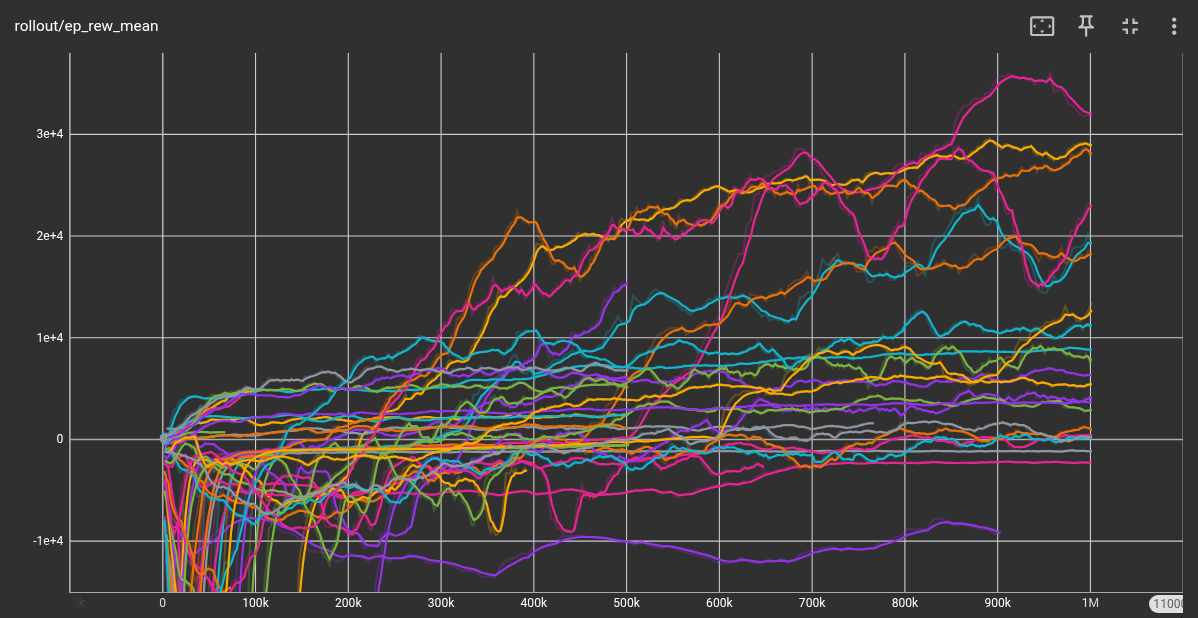
\includegraphics[width=0.48\textwidth]{images/ep_rew_mean.png}\hfill
    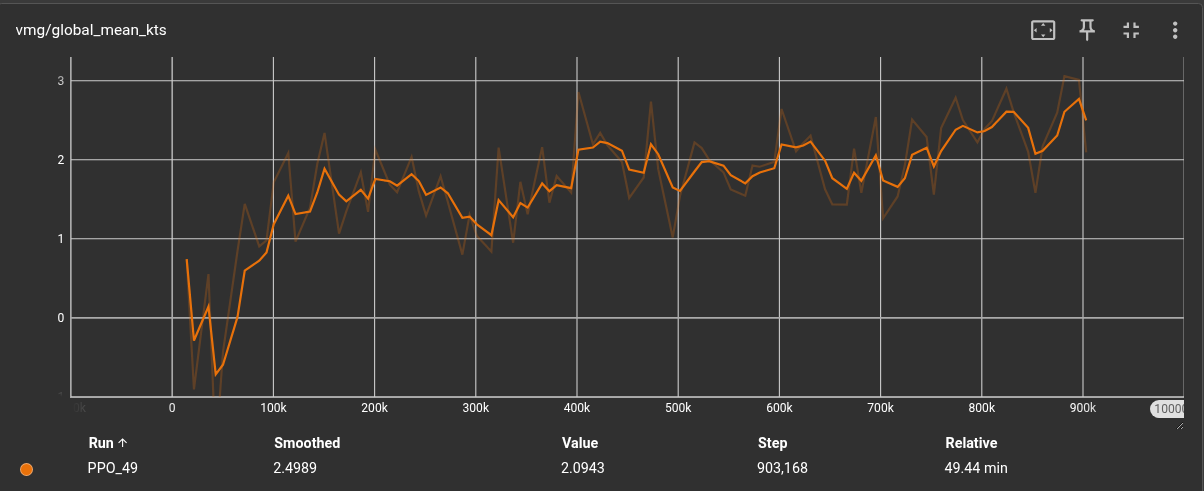
\includegraphics[width=0.48\textwidth]{images/global_mean_kts.png}
    \caption{Training metrics tracked via TensorBoard. The left graph illustrates the learning curve via the mean episodic reward, while the right graph demonstrates the agents successfully learning to maximize their average Velocity Made Good (VMG) over time.}
    \label{fig:tensorboard}
\end{figure}

A qualitative analysis of the rendered races (see the supplementary video) revealed several sophisticated emergent behaviors:
\begin{itemize}
    \item \textbf{Wind Adaptation:} Agents learned to autonomously perform tactical tacks and gybes in response to wind shifts generated by the 2D random walk model, optimizing their trajectory to stay in the favored wind phase.
    \item \textbf{Close-Quarters Tactics:} Thanks to the Time-To-Collision (TTC) penalty and the asymmetrical Rule 10 penalties, the boats developed realistic crossing behaviors. For instance, a boat on a port tack learned to bear away or tack early to avoid a catastrophic penalty when encountering a starboard-tack opponent.
    \item \textbf{Gate Maneuvering:} The agents successfully learned the complex sequence of actions required to round the top mark, smoothly transitioning from an upwind displacement regime to a downwind foiling trajectory without excessively losing speed.
\end{itemize}

\begin{figure}[htpb]
    \centering
    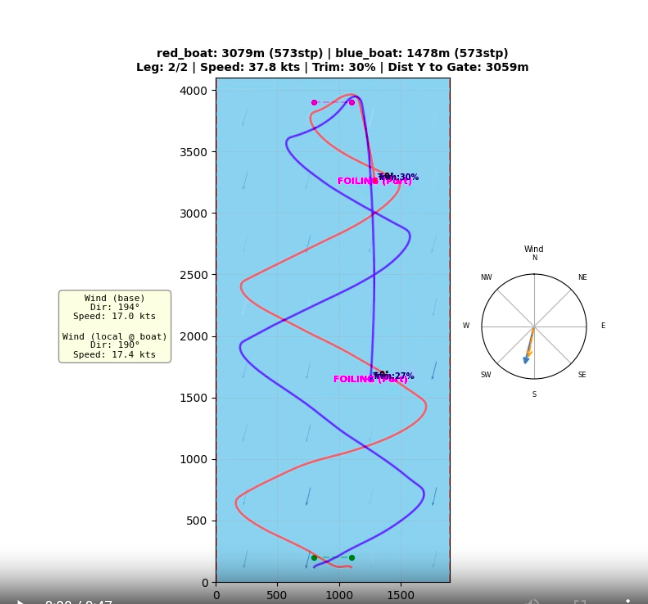
\includegraphics[width=0.8\textwidth]{images/screenshot_navigation.png}
    \caption{A frame from the simulation showing the end of the race. The overall trajectory of the boats highlights their ability to perform complex tactical maneuvers, such as tacking and gate roundings, to optimize their Velocity Made Good (VMG) across the entire course.}
    \label{fig:trajectory}
\end{figure}

\section{Conclusions and Future Work}
In this project, we successfully applied Multi-Agent Reinforcement Learning to the highly complex domain of competitive sailing. Our \textit{CoppaAmerica Multiagent} framework effectively bridges the gap between raw physical simulation (foiling, VPP) and strategic decision-making. The trained PPO agents demonstrated the ability to continuously control rudder and sail trim, react to stochastic wind fields, and adhere to fundamental racing rules, ultimately achieving a highly competitive success rate.

While the current results are extremely promising, several avenues for future research remain open. A natural extension would involve scaling the simulator to support fleet racing with more than two boats, significantly increasing the complexity of the multi-agent interactions. Additionally, refining the aerodynamic models---for example, explicitly modeling the wind shadow (blanketing effect) cast by a boat's sails onto its opponents---would further elevate the tactical realism of the simulator.

\begin{thebibliography}{9}
\bibitem{ppo} 
John Schulman, Filip Wolski, Prafulla Dhariwal, Alec Radford, Oleg Klimov. 
\textit{Proximal Policy Optimization Algorithms}. 
arXiv preprint arXiv:1707.06347 (2017).

\bibitem{pettingzoo} 
J. K. Terry, Benjamin Black, Nathaniel Grammel, Mario Jayakumar, Ananth Hari, Ryan Sullivan, Luis S. Santos, Clemens Dieffendahl, Caroline Horsch, Rodrigo Perez-Vicente, et al. 
\textit{PettingZoo: Gym for Multi-Agent Reinforcement Learning}. 
Advances in Neural Information Processing Systems (NeurIPS) 34 (2021).

\bibitem{sb3} 
Antonin Raffin, Ashley Hill, Adam Gleave, Anssi Kanervisto, Maximilian Ernestus, Noah Dormann. 
\textit{Stable-Baselines3: Reliable Reinforcement Learning Implementations}. 
Journal of Machine Learning Research (JMLR) 22(268):1-8 (2021).
\end{thebibliography}

\end{document}
